\section{Behaviors}
\label{sec:Behaviors}
% Owner: Jani
% Reviewed:
%
The addressed solution provides in its default setting already several behaviors for merchants as well as the consumers. The former include known rule-based strategies like the ``Gas Station strategy'', ``Be the n-cheapest'', ``fix pricing'' as well as a first data-driven approach implementing a pricing strategy based on logistic regression \citep{hosmer2013applied}.

%
\begin{figure}[h]
    \centering
    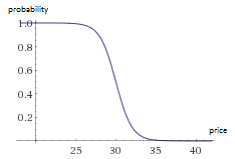
\includegraphics[width=0.25\textwidth]{images/sigmoid.png}
    \caption{Sigmoid distribution as consumer behavior}
    \label{fig:sigmoid_distribution}
\end{figure}
%

Additionally, a consumer is included in the deployment implementing several buying behaviors which can be chosen, weighted and reconfigured on-the-fly. Those behaviors range from very subtle approaches like buying the n-cheapest, first, most expensive or simple random offers on the marketplace up to more sophisticated methods trying to imitate more complex consumer situations. A sigmoid distribution with twice of the producer price as mean (see fig. \ref{fig:sigmoid_distribution}) is available through the default settings as well as a logit behavior.

The logit behavior implements a logistic regression with feature scaling and calculates for each offer the buying probability based on the feature coefficients provided in the behavior settings. Based on this buying probability for each offer, the consumer will actually choose an offer to buy. In this way, potential consumer behavior can be learned on real world data and imitated in the simulation solution.

The default settings for the logit behavior holds coefficients which were extracted from a real world use case provided by a big book retail company. For deeper insights in the concepts of logistic regression, the reader is kindly referred to \citet{hosmer2013applied} elaboration.

%
\begin{figure}[h]
    \centering
    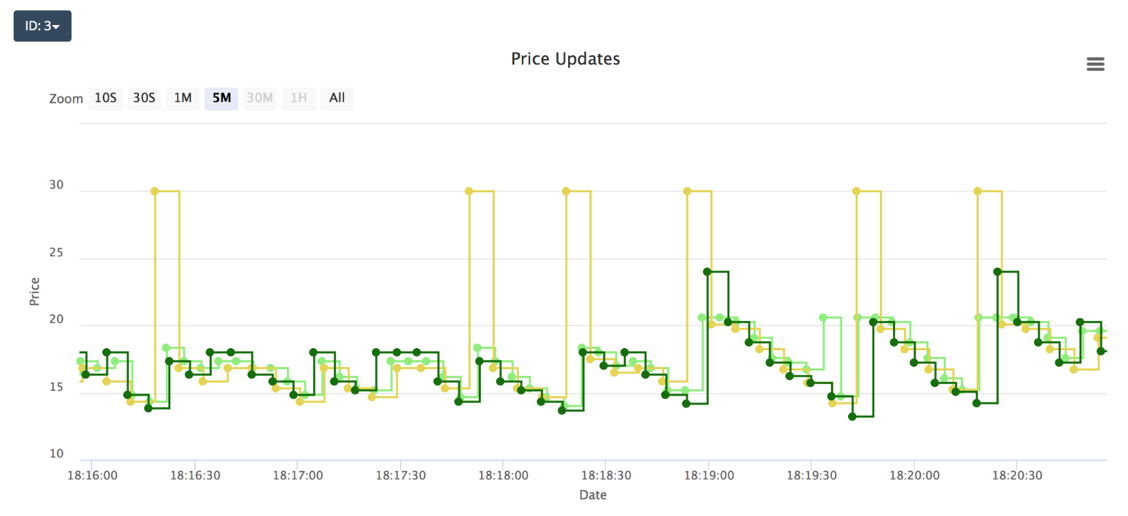
\includegraphics[width=0.5\textwidth]{images/price_graphs_v2.png}
    \caption{Price Graphs}
    \label{fig:price_graphs_v2}
\end{figure}
%

%
\subsection{Logistic Regression}
\label{sec:Logistic_Regression}
% Owner: 
% Reviewed:
%
Logistic regression is a regression model where the dependent variable -- in our case the selling of an offer -- is categorical. This categorization outcome must be discrete and should be dichotomous in nature simply expressed by a boolean whether a purchase happened or not. To determine this, this behavior consumes features and their coefficients can be altered within runtime and will then be applied to the next calculation iteration taking place. The describing hashmap of features and their coefficients contains only available features which are already implemented otherwise they will be ignored.